\scanpage{365}
$P^i$ op stables \unsure{construite|construites} par Steenrod.
\mspage{4}

$p=2$
\[
\mathbb F_2[\underline{\operatorname{Sq}^i}]\qquad i\geq0
\]
\[
\operatorname{Sq}^0=1\qquad(\operatorname{Sq}^1=\beta)\quad\text{rel d'\unsure{Adem|Aden}}
\]
$\deg\operatorname{Sq}^i=i$

\margin{$p\quad2$}
\deleted{$\operatorname{Sq}^1\operatorname{Sq}^2=\operatorname{Sq}$}
\[
\operatorname{Sq}^1\operatorname{Sq}^2=\operatorname{Sq}^3+\operatorname{Sq}^2\operatorname{Sq}^1\qquad(?)
\]
etc --
\figure{\begin{tikzpicture}\draw (0,0) .. controls (.4,.02) and (.6,0) .. (.8,-.02);\end{tikzpicture}}

Formule de Cartan:
\[
P^i(x\times y)=\sum_{j\geq0}P^j(x)P^{i-j}(y)
\]
\[
P^I=\beta^{\epsilon_0}P^{\eta_1}\beta^{\unsure{\epsilon_1|\epsilon_i}}P^{\eta_2}\ldots
\qquad I\unsure{\sim|=}(\epsilon_0,\eta_1,\epsilon_1,\eta_2,\ldots)
\]
\margin{deg $I$ de manière evidente\par
excès $e(I)=\text{``}\eta_1-\sum_{i>1}\eta_i\text{''}$}
\[
\epsilon_i=0,1\qquad\eta_i\geq0
\]
admissible
\[
\eta_i\geq p\eta_{i+1}+\epsilon_i
\]
les $P^I$ \unsure{admissible|admissibles} forment une $\mathbb F_p$ base.
\figure{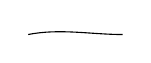
\begin{tikzpicture}\draw (0,0) .. controls (.4,.08) and (.8,0) .. (1.2,0);\end{tikzpicture}}
\diagram{\begin{tikzcd}[column sep=large,execute at end picture={\draw (-1.3,0) ellipse (.45 and .35);}]
A\arrow[r]&H^*(\unsure{K|\kappa}(\mathbb F_p,n),\mathbb F_p)\\
x&x\unsure{\iota_n|i_n}
\end{tikzcd}}

\uline{Theorème}.
\margin{Serre ($p=2$)}
\[
H^*(\unsure{K|\kappa}(\mathbb F_p,n),\mathbb F_p)=
\]
Algebre anticommutative libre sur $\mathbb F_p$ engendrée par \unsure{le|les} \uline{monomes \unsure{admissible|admissibles}} d'excès $<n$.
\[
H_*(\underline{\unsure{K|\kappa}(\mathbb F_p,n)},\mathbb F_p)=
\]
Alg anticom à puiss \unsure{divisée|divisées} universelle engendrée par \unsure{le|les} \unsure{element|elements} duaux.
\mspage{366}
